% !TeX program = pdflatex
% !BIB program = bibtex
% Template LaTeX file for DAFx-19 papers
%
% To generate the correct references using BibTeX, run
%     latex, bibtex, latex, latex
% modified...
% - from DAFx-00 to DAFx-02 by Florian Keiler, 2002-07-08
% - from DAFx-02 to DAFx-03 by Gianpaolo Evangelista
% - from DAFx-05 to DAFx-06 by Vincent Verfaille, 2006-02-05
% - from DAFx-06 to DAFx-07 by Vincent Verfaille, 2007-01-05
%                          and Sylvain Marchand, 2007-01-31
% - from DAFx-07 to DAFx-08 by Henri Penttinen, 2007-12-12
%                          and Jyri Pakarinen 2008-01-28
% - from DAFx-08 to DAFx-09 by Giorgio Prandi, Fabio Antonacci 2008-10-03
% - from DAFx-09 to DAFx-10 by Hannes Pomberger 2010-02-01
% - from DAFx-10 to DAFx-12 by Jez Wells 2011
% - from DAFx-12 to DAFx-14 by Sascha Disch 2013
% - from DAFx-15 to DAFx-16 by Pavel Rajmic 2015
% - from DAFx-16 to DAFx-17 by Brian Hamilton 2016
% - from DAFx-18 to DAFx-19 by Dave Moffat 2019
%
% Template with hyper-references (links) active after conversion to pdf
% (with the distiller) or if compiled with pdflatex.
%
% 20060205: added package 'hypcap' to correct hyperlinks to figures and tables
%                      use of \papertitle and \paperauthorA, etc for same title in PDF and Metadata
%
% 1) Please compile using latex or pdflatex.
% 2) If using pdflatex, you need your figures in a file format other than eps! e.g. png or jpg is working
% 3) Please use "paperftitle" and "pdfauthor" definitions below

%------------------------------------------------------------------------------------------
%  !  !  !  !  !  !  !  !  !  !  !  ! user defined variables  !  !  !  !  !  !  !  !  !  !  !  !  !  !
% Please use these commands to define title and author(s) of the paper:
\def\papertitle{Real-time Physical Model for Analog Tape Machines}
\def\paperauthorA{Jatin Chowdhury}

% Authors' affiliations have to be set below

%------------------------------------------------------------------------------------------
\documentclass[twoside,a4paper]{article}
\usepackage{dafx_19}
\usepackage{amsmath,amssymb,amsfonts,amsthm}
\usepackage{euscript}
\usepackage[latin1]{inputenc}
\usepackage[T1]{fontenc}
\usepackage{ifpdf}

\usepackage[english]{babel}
\usepackage{caption}
\usepackage{subfig} % or can use subcaption package
\usepackage{color}

\setcounter{page}{1}
\ninept

\usepackage{times}
% Saves a lot of ouptut space in PDF... after conversion with the distiller
% Delete if you cannot get PS fonts working on your system.

% pdf-tex settings: detect automatically if run by latex or pdflatex
\newif\ifpdf
\ifx\pdfoutput\relax
\else
   \ifcase\pdfoutput
      \pdffalse
   \else
      \pdftrue
\fi

\ifpdf % compiling with pdflatex
  \usepackage[pdftex,
    pdftitle={\papertitle},
    pdfauthor={\paperauthorA},
    colorlinks=false, % links are activated as colror boxes instead of color text
    bookmarksnumbered, % use section numbers with bookmarks
    pdfstartview=XYZ % start with zoom=100% instead of full screen; especially useful if working with a big screen :-)
  ]{hyperref}
  \pdfcompresslevel=9
  \usepackage[pdftex]{graphicx}
  \usepackage[figure,table]{hypcap}
\else % compiling with latex
  \usepackage[dvips]{epsfig,graphicx}
  \usepackage[dvips,
    colorlinks=false, % no color links
    bookmarksnumbered, % use section numbers with bookmarks
    pdfstartview=XYZ % start with zoom=100% instead of full screen
  ]{hyperref}
  % hyperrefs are active in the pdf file after conversion
  \usepackage[figure,table]{hypcap}
\fi
\usepackage{cleveref}

\title{\papertitle}

\affiliation{
\paperauthorA \,}
{\href{http://ccrma.stanford.edu}{Center for Computer Research in Music and Acoustics} \\ Stanford University \\ Palo Alto, CA \\ {\tt \href{mailto:jatin@ccrma.stanford.edu}{jatin@ccrma.stanford.edu}}}

\begin{document}
% more pdf-tex settings:
\ifpdf % used graphic file format for pdflatex
  \DeclareGraphicsExtensions{.png,.jpg,.pdf}
\else  % used graphic file format for latex
  \DeclareGraphicsExtensions{.eps}
\fi

\maketitle

\section{Abstract}
For decades, analog magnetic tape recording was the most popular
method for recording music, but has been replaced over the past 30 years first by
DAT tape, and then by DAWs \cite{Kadis}. Despite being replaced
by higher quality technology,
many have sought to recreate a "tape" sound through digital effects, despite
the distortion, tape "hiss", and other oddities analog tape produced.
The following describes
a physical modelling process for an analog tape machine,
starting from basic physical principles.
\newline\newline
"Whatever you now find weird, ugly, uncomfortable, and nasty
about a new medium will surely become its signature. CD distortion, the jitteriness
of digital video, the crap sound of 8-bit - all of these will be cherished
and emulated as soon as they can be avoided." -Brian Eno \cite{Eno}.

\section{Continuous Time System}
Audio recorded to and played back from a tape machine can be thought of as going
through three distinct processors: the record head, tape magnetisation, and the play
head.

\subsection{The Record Head}
For an instantaneous input current $I(t)$, the magnetic field output of the record 
head is given as a function of distance along the tape 'x', and depth into 
the tape 'y' (Karlqvist medium field approximation) \cite{1994tmr..book.....B}.

\begin{multline}
    H_x(x,y) = \frac{1}{\pi} H_0 \Big(\tan^{-1} \Big(\frac{(g/2) + x}{y} \Big) + \\
    \tan^{-1} \Big(\frac{(g/2) - x}{y} \Big) \Big)
    \label{eq1}
\end{multline}
\begin{equation}
    H_y(x,y) = \frac{1}{2 \pi} H_0 \ln \Big(\frac{((g/2) - x)^2 + y^2}{((g/2) + x)^2 + y^2} \Big)
    \label{eq2}
\end{equation}
%
where $g$ = head gap, and $H_0$ = deep gap field, given by:

\begin{equation}
    H_0 = \frac{NEI}{g}
\end{equation}
%
where $N$ = number of turns coils of wire around the head, and $E$ = head 
efficiency which can be calculated by:

\begin{equation}
    E = \frac{1}{1 + \frac{l  A_g}{\mu_r g} \int_{core} \frac {d \vec{l}}{A(l)}}
\end{equation}
%
where $A_g$ is the gap area, $\mu_r$ is the core permeability relative to 
free space ($\mu_0$), $g$ if the gap width, and $A(l)$ is the cross-sectional 
area of the core as a function of length.

\subsection{Tape Magnetisation}
The magnetic field being recorded to tape can be described using 
a hysteresis loop, as follows \cite{1994tmr..book.....B}:

\begin{equation}
    \vec{M}(x,y) = F_{Loop}(\vec{H}(x,y))
\end{equation}
%
where $F_{Loop}$ is a generalized hysteresis function.
\newline\newline
Using the Jiles-Atherton magnetisation model, the following
differential equation describes magnetisation 'M' as a function 
of magnetic field 'H' \cite{Hysteresis}:

\begin{equation}
    \frac{dM}{dH} = \frac{(1-c) \delta_M (M_{an} - M)}{(1-c) \delta k - \alpha (M_{an} - M)} + c \frac{dM_{an}}{dH}
    \label{eq5}
\end{equation}
%
where $c$ is the ration of normal and anhysteric initial susceptibilities,
$k$ is a measure of the width of the hysteresis
loop, $\alpha$ is a mean field parameter, representing inter-domain
coupling, and

\begin{equation}
    \delta = \begin{cases}
        1 & \text{if H is increasing} \\
        -1 & \text{if H is decreasing}
    \end{cases}
\end{equation}
\begin{equation}
    \delta_M = \begin{cases}
        1 & \text{if $\delta$ and $M_{an} - M$ have the same sign} \\
        0 & \text{otherwise}
    \end{cases}
\end{equation}
%
$M_{an}$ is the anisotropic magnetisation given by:

\begin{equation}
    M_{an} = M_s L \Big( \frac{H + \alpha M}{a} \Big)
\end{equation}
%
where $M_s$ is the magnetisation saturation, $a$ characterizes the shape
of the anhysteric magnetisation and $L$ is the Langevin function:

\begin{equation}
    L(x) = \coth (x) - \frac{1}{x}
\end{equation}

\subsection{Play Head}
\subsubsection{Ideal Playback Voltage}
The ideal playback voltage as a function of tape magnetisation is given by
\cite{1994tmr..book.....B}:

\begin{equation}
    V(x) =  NWEv \mu_0 \int_{-\infty}^{\infty} dx' \int_{-\delta/2}^{\delta/2} dy' \vec{h}(x' + x, y') \cdot \frac{\vec{M}(x', y')}{dx}
    \label{eq11}
\end{equation}
%
where $N$ = number of turns of wire, $W$ = width of the playhead, $E$ = playhead
efficiency, $v$ = tape speed, and $\mu_0$ is the permeability of free space.
Note that $V(x) = V(vt)$ for constant $v$. $\vec{h}(x, y)$ is defined as:

\begin{equation}
    \vec{h} (x, y) \equiv \frac{\vec{H} (x, y)}{NIE}
    \label{eq12}
\end{equation}
%
where $\vec{H} (x, y)$ can be calculated by \cref{eq1,eq2}.

\subsubsection{Loss Effects}
There are several frequency-dependent loss effects associated with playback,
described as follows \cite{Kadis}:

\begin{equation}
    V(x) = V_0(x) [e^{-kd}] \Big[\frac{1 - e^{-k \delta}}{k \delta} \Big] \Big[\frac{\sin (kg /2)}{kg/2} \Big]
    \label{eq:lossEffects}
\end{equation}
%
for sinusoidal input, where $k$ = wave number, $d$ is the distance between the tape and the playhead,
$g$ is the gap width of the play head, and $\delta$ is the thickness of the tape.

\section{Digitizing the System}
\subsection{Record Head}
For simplicity, let us assume,
\begin{equation}
    \vec{H}(x,y,t) = \vec{H}(0,0,t)
\end{equation}
%
In this case $H_y \equiv 0$, and $H_x \equiv H_0$. Thus,
\begin{equation}
    H(t) = \frac{NEI(t)}{g}
    \label{eq15}
\end{equation}
%
or,
\begin{equation}
    \hat{H}(n) = \frac{NE\hat{I}(n)}{g}
\end{equation}

\subsection{Hysteresis}
Beginning from \cref{eq5}, we can find the derivative of $M$ w.r.t. time,
as in \cite{Hysteresis}:
\begin{equation}
    \frac{dM}{dt} = \frac{\frac{(1-c) \delta_M (M_sL(Q) - M)}{(1-c) \delta k - \alpha (M_sL(Q) - M)} \frac{dH}{dt} + c \frac{M_s}{a} \frac{dH}{dt} L'(Q)}{1 - c \alpha \frac{M_s}{a} L'(Q)}
    \label{eq:dmdt}
\end{equation}
%
where $Q = \frac{H + \alpha M}{a}$, and

\begin{equation}
    L'(x) = \frac{1}{x^2} - \coth^2(x) + 1
\end{equation}
%
Note that \cref{eq:dmdt} can also be written in the general form for non-linear
Ordinary Differential Equations:
\begin{equation}
    \frac{dM}{dt} = f(t,M,\vec{u})
\end{equation}
where $\vec{u} = \begin{bmatrix}
    H \\
    \dot{H}
    \end{bmatrix}$.
\newline\newline
Using the trapezoidal rule for derivative approximation, we find:

\begin{equation}
    \dot{\hat{H}}(n) = 2\frac{\hat{H}(n) - \hat{H}(n-1)}{T} - \dot{\hat{H}}(n-1)
\end{equation}
%
We can use the Runge-Kutta 4th order method \cite{Yeh} to find an explicit solution
for $\hat{M}(n)$:
\begin{align}
\begin{split}
    k_1 &= T f \Big(n-1, \hat{M}(n-1), \hat{\vec{u}}(n-1) \Big)\\
    k_2 &= T f \Big(n - \frac{1}{2}, \hat{M}(n-1) + \frac{k_1}{2}, \hat{\vec{u}}  \Big(n-\frac{1}{2} \Big) \Big)\\
    k_3 &= T f \Big(n- \frac{1}{2}, \hat{M}(n-1) + \frac{k_2}{2}, \hat{\vec{u}} \Big(n-\frac{1}{2} \Big) \Big)\\
    k_4 &= T f \Big(n, \hat{M}(n-1) + k_3, \hat{\vec{u}}(n) \Big)\\
    \hat{M}(n) &= \hat{M}(n-1) + \frac{k_1}{6} + \frac{k_2}{3} + \frac{k_3}{3} + \frac{k_4}{6}
\end{split}
\end{align}
%
We use linear interpolation to find the half-sample values used to calculate $k_2$ and $k_3$.

\subsubsection{Numerical Considerations}
To account for rounding errors in the Langevin function for values close to 
zero, we use the following approximation about zero, as in \cite{Hysteresis}:
\begin{equation}
    L(x) = \begin{cases}
        \coth(x) - \frac{1}{x} & \text{for $|x| > 10^{-4}$} \\
        \frac{x}{3} & \text{otherwise}
    \end{cases}
\end{equation}
\begin{equation}
    L'(x) = \begin{cases}
        \frac{1}{x^2} - \coth^{2}(x) + 1 & \text{for $|x| > 10^{-4}$} \\
        \frac{1}{3} & \text{otherwise}
    \end{cases}
\end{equation}

\subsubsection{Simulation}
The digitized hysteresis loop was implemented and tested offline
in \texttt{Python}, using the constants $M_s$, $a$, $\alpha$, $k$,
and $c$ from \cite{JilesAtherton1986}. For a sinusoidal input signal
with frequency 2kHz, and varying amplitude from 800 - 2000 Amperes per
meter, the following plot shows the Magnetisation output.

\begin{figure}[ht]
    \center
    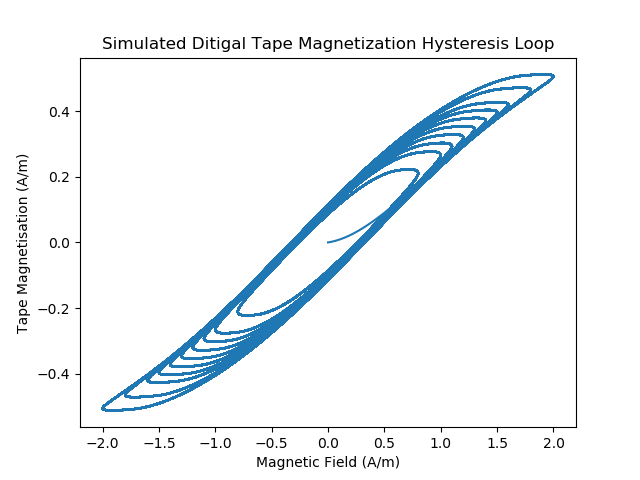
\includegraphics[width=3in]{../Simulations/Sim2-M_H.png}
    \caption{\label{flowchart}{\it Digitized Hysteresis Loop Simulation}}
\end{figure}
%
\subsection{Play Head}
By combining \cref{eq11} with \cref{eq12,eq15}, we get:
\begin{equation}
    V(t) =  NWEv \mu_0  g M(t)
\end{equation}
%
or,
\begin{equation}
    \hat{V}(n) =  NWEv \mu_0  g \hat{M}(t)
\end{equation}
%
The loss effects described in \cref{eq:lossEffects}
can be modelled as a series of digital filters.

\subsection{Oversampling}
To reduce frequency aliasing caused by the hysteresis non-linearity,
we recommend oversampling by at least 4x.
%
%\section{Determining System Parameters}
%\subsection {Tape Machine Parameters}
%%@TODO: Do I need this section?
%\subsubsection {Record Head}
%The input current to the record head is approximately 0.1 mA peak-to-peak
%\cite{RefManual}. Plugging into equation (16)
%
%g = 20 microns, N = 100, E = 0.1
%
%gives a peak-to-peak field amplitude of 5E5 A/m
%
%\subsubsection{Play Head}
%N = 100, W = 0.25in = 6.3e-3m, v = 7 ips = 0.18 m/s,
%g = 20 microns, mu = 12.57e-7
%
%Gain of play head = 2.85e-14
\section{System Parameters}
\subsection {Tape Parameters}
For the tape hysteresis \cref{eq:dmdt}, following parameters are necessary:
\begin{itemize}
\item Magnetic Saturation ($M_s$): For Ferric Oxide ($\gamma F_2O_3$)
magnetic tape as would typically be used for a reel-to-reel machine,
the magnetic saturation is $3.5e5$ (A/m) \cite{jilesBook}
\item Hysteresis Loop Width ($k$): For soft materials, $k$ can be approximated
as the coercivity, $H_c$ \cite{Jiles1992}. For Ferric Oxide, $H_c$ is approximately
$27$ kA/m \cite{jilesBook}.
\item a: Knowing the coercivity and remnance magnetism of Ferric Oxide
\cite{jilesBook}, we can calculate $a$ = 22  kA/m by the method described includegraphics
\cite{Jiles1992}
\item c: From \cite{Jiles1992}, $c$ = 1.7e-1.
\item alpha: From \cite{Jiles1992}, alpha = 1.6e-3
\end{itemize}

\subsection{Tape Bias}
A typical analog recorder adds a high-frequency "bias"
current to the signal to avoid the "deadzone" effect when the input signal
crosses zero, as well as to linearize the output. The input
current to the record head can be given by
\cite{Camras:1987:MRH:27189}:
\begin{equation}
    \hat{I}_{head}(n) = \hat{I}_{in}(n) + B \cos(2 \pi f_{bias} n T)
\end{equation}
%
Where the amplitude of the bias current $B$ is usually
about one order of magnitude larger than the input,
and the bias frequency $f_{bias}$ is well above the
audible range. The output signal can be
recovered after the recording and playback processes
by subtracting out the bias current.

\subsection{Tape Speed}
The frequency response of the playback from a tape
recorder is also dependent on the tape speed. Faster
speeds typically correspond to better high-frequency
response. In this case, we model the tape speed response
as a simple low-pass filter.

%\newpage
\nocite{*}
\bibliographystyle{IEEEbib}
\bibliography{references}

\end{document}
